\section{Job Shops} \label{sec:9}
In a job shop, each job has its own route to follow through the machines. 
This is a more general case of the flow job, where each job followed 
the same route. We will focus on the makespan objective, and describe 
formulations of the job shop problem as disjunctive graphs. We then 
describe two approaches to solving the problem: a branch and bound approach, 
and a popular and effective heuristic. 

\subsection{Disjunctive Programming and Branch and Bound} \label{subsec:9.1}
We first say a few words on active schedules and semi-active schedules.

\begin{defn}{defn:9.1}
    We say that a schedule is {\bf active} if it is not possible to 
    construct another schedule by changing the order of processing on the 
    machines and having at least one task finishing earlier without 
    any task finishing later. (Informally, when a schedule is active and there 
    are ``holes'' in the Gantt chart, then we cannot fit any of the later jobs 
    into these holes.)

    We say that a schedule is {\bf semi-active} if no task can be 
    completed earlier without changing the order of processing on any 
    one of the machines. 
\end{defn}

\begin{exmp}{exmp:9.2}
    Consider the following job shop with $3$ machines and $2$ jobs, where 
    both jobs must be processed last on machine $2$.  
    \begin{align*}
        \begin{array}{c|c|c}
            \text{Job} & \text{Machine Sequence} & \text{Processing Times} \\ \hline 
            1 & 1, 2 & p_{11} = 1,\, p_{21} = 3 \\ 
            2 & 3, 2 & p_{32} = 2,\, p_{22} = 3
        \end{array}
    \end{align*}
    Then the following schedule is active as reversing the sequence 
    of the two jobs on machine $2$ postpones the processing of job $2$. 
    However, the schedule is neither non-delay nor optimal, since machine 
    $2$ remains idle until time $2$ while there is a job available for processing 
    at time $1$. 
    \begin{center} 
        \begin{tikzpicture}[/pgfgantt/y unit chart=0.65cm] 
            \begin{ganttchart}[
                title/.style={draw=none},
                canvas/.append style={draw=none}, 
                bar top shift=0.1, bar height=0.6,
                y unit title=0.65cm
            ]{1}{8}
                \ganttbar{Machine 1}{1}{1} \ganttbar[inline]{1}{1}{1} \\ 
                \ganttbar{Machine 2}{3}{5} \ganttbar[inline]{2}{3}{5} \ganttbar[inline]{1}{6}{8} \\ 
                \ganttbar{Machine 3}{1}{2} \ganttbar[inline]{2}{1}{2} \\ 
                \gantttitlelist{1,...,8}{1}
            \end{ganttchart}
        \end{tikzpicture}
    \end{center} 
    \vspace{-0.5cm}
    Consider now the job shop which has the same routing as above but 
    the processing times are now $p_{11} = p_{21} = 1$ and 
    $p_{32} = p_{22} = 2$. The following schedule is a semi-active schedule.
    However, it is not active as job $1$ can be processed on machine $2$ 
    without delaying the processing of job $2$ on machine $2$.  
    \begin{center} 
        \begin{tikzpicture}[/pgfgantt/y unit chart=0.65cm] 
            \begin{ganttchart}[
                title/.style={draw=none},
                canvas/.append style={draw=none}, 
                bar top shift=0.1, bar height=0.6,
                y unit title=0.65cm
            ]{1}{5}
                \ganttbar{Machine 1}{1}{1} \ganttbar[inline]{1}{1}{1} \\ 
                \ganttbar{Machine 2}{3}{4} \ganttbar[inline]{2}{3}{4} \ganttbar[inline]{1}{5}{5} \\ 
                \ganttbar{Machine 3}{1}{2} \ganttbar[inline]{2}{1}{2} \\ 
                \gantttitlelist{1,...,5}{1}
            \end{ganttchart}
        \end{tikzpicture}
    \end{center} 
    \vspace{-0.4cm}
\end{exmp}

The $(J_m~||~C_{\max})$ can be represented using a nice disjunctive graph. 
Consider a directed graph $G$ with a set of nodes $N$ and two sets of 
arcs $A$ and $B$. The nodes $N$ correspond to all the operations $(i, j)$ 
that must be performed on the $n$ jobs. The {\bf conjunctive} arcs $A$
represent the routes of the jobs. That is, if the arc $(i, j) \to (k, j)$ 
is a part of $A$, then job $j$ has to be processed on machine $i$ before 
it is processed on machine $k$. Two operations that belong to different 
jobs but the same machine are joined by a {\bf disjunctive} arc, 
which has no direction given to it yet. The disjunctive arcs $B$ form 
$m$ cliques for each machine, and all operations in the same clique 
have to be done on the same machine. Each node has cost the processing 
time of the operation represented by that node. In addition, there is a 
source $0$ and a sink $\star$, which are dummy nodes. The source node $0$ 
has $n$ conjunctive arcs emanating to the first operations of the $n$ jobs, 
and the sink node has $n$ conjunctive arcs coming in from the last operations. 
This graph is denoted $G = (N, A, B)$. 
\begin{center}
    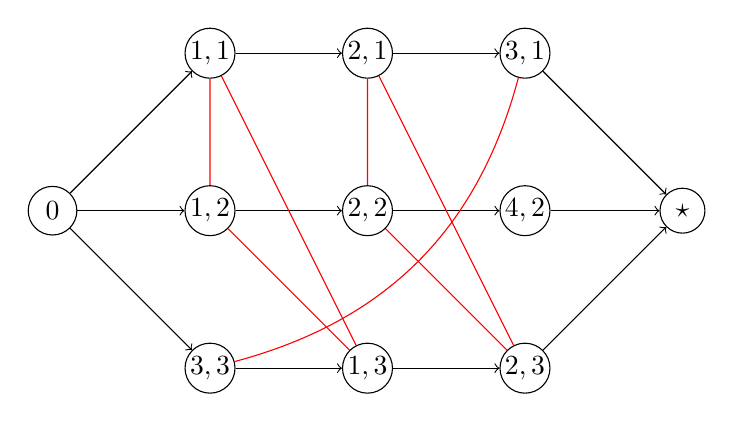
\begin{tikzpicture}              
        \node [circle, draw=black] (0) at (0, 0) {$0$}; 
        \node [circle, draw=black, inner sep=0.5pt] (11) at (2, 2) {$1, 1$}; 
        \node [circle, draw=black, inner sep=0.5pt] (12) at (2, 0) {$1, 2$}; 
        \node [circle, draw=black, inner sep=0.5pt] (33) at (2, -2) {$3, 3$}; 
        \node [circle, draw=black, inner sep=0.5pt] (21) at (4, 2) {$2, 1$}; 
        \node [circle, draw=black, inner sep=0.5pt] (22) at (4, 0) {$2, 2$}; 
        \node [circle, draw=black, inner sep=0.5pt] (13) at (4, -2) {$1, 3$}; 
        \node [circle, draw=black, inner sep=0.5pt] (31) at (6, 2) {$3, 1$}; 
        \node [circle, draw=black, inner sep=0.5pt] (42) at (6, 0) {$4, 2$}; 
        \node [circle, draw=black, inner sep=0.5pt] (23) at (6, -2) {$2, 3$};
        \node [circle, draw=black] (star) at (8, 0) {$\star$};
        
        \draw [->] (0) -- (11); \draw [->] (0) -- (12); \draw [->] (0) -- (33);
        \draw [->] (11) -- (21); \draw [->] (21) -- (31); \draw [->] (31) -- (star);
        \draw [->] (12) -- (22); \draw [->] (22) -- (42); \draw [->] (42) -- (star);
        \draw [->] (33) -- (13); \draw [->] (13) -- (23); \draw [->] (23) -- (star);
        \draw [color=red] (11) -- (12) -- (13) -- (11);
        \draw [color=red] (21) -- (22) -- (23) -- (21);
        \draw [red, bend right] (33) edge (31);
    \end{tikzpicture} 
\end{center}

A feasible schedule corresponds to selecting a direction for each 
disjunctive arc such that the resulting graph is acyclic. This implies that 
the selection of direction for each clique must be acyclic. Such a 
selection determines the sequence in which the operations are to be 
performed on that machine. If $D$ denotes the subset of the selected 
disjunctive arcs and $G(D)$ is the graph containing the conjunctive 
arcs together with the selected disjunctive arcs, then $D$ corresponds 
to a feasible schedule if and only if $G(D)$ contains no directed cycles. 

The makespan of a feasible schedule is determined by the longest path 
in $G(D)$ from the source $0$ to the sink $\star$. This longest path 
consists of a set of operations of which the first starts at time $0$ 
and the last finishes at the time of the makespan. Each operation 
on this path is immediately followed by either the next operation on the 
same machine or the next operation of the same job on another machine. 
Thus, the problem of minimizing the makespan is reduced to finding a 
selection of disjunctive arcs that minimizes the length of the longest 
path (that is, the {\bf critical} path). 

We now give a so-called disjunctive programming formulation for minimizing 
the makespan in a job shop. This formulation is closely related to 
the disjunctive graph representation of the job shop. 

Let $y_{ij}$ denote the starting time of operation $(i, j)$. Recall 
that the set $N$ denotes the set of all operations $(i, j)$, and 
the set $A$ contains all routing constraints $(i, j) \to (k, j)$ that 
require job $j$ to be processed on machine $i$ before it is processed on 
machine $k$. Then the following program minimizes the makespan. 
\begin{align*}
    \min\quad & C_{\max} \\ 
    \text{s.t.}\quad & y_{kj} - y_{ij} \geq p_{ij}, && \text{for all } (i, j) \to (k, j) \in A, \\ 
    & C_{\max} - y_{ij} \geq p_{ij}, && \text{for all } (i, j) \in N, \\ 
    & y_{ij} - y_{i\ell} \geq p_{i\ell} \text{ or } y_{i\ell} - y_{ij} \geq p_{ij}, 
        && \text{for all } (i, \ell) \text{ and } (i, j),\; i = 1, \dots, m, \\ 
    & y_{ij} \geq 0, && \text{for all } (i, j) \in N. 
\end{align*}
The first set of constraints ensure that operation $(k, j)$ cannot start before 
operation $(i, j)$ is completed. The third set of constraints are called the 
disjunctive constraints, and ensure that some ordering exists among operations 
of different jobs that have to be processed on the same machine. Because of 
these constraints, this formulation is referred to as a disjunctive programming 
formulation. 

Of course, the fact that a scheduling problem can be formulated as a 
disjunctive program does not imply that there is a standard solution 
procedure available that will work satisfactorily. Minimizing the makespan 
in a job shop is a very hard problem and solution procedures are either 
based on enumeration or on heuristics. 

To obtain an optimal solution, we require branch and bound methods. 
The branching as well as the bounding procedures that are applicable to this 
problem are usually of a special design. In this case, we will consider 
active schedules. It can be shown that there exists among all possible 
schedules an active schedule that minimizes the makespan. 

A branching schedule that is often used is based on the generation of 
all active schedules. All such active schedules can be generated by a 
simple algorithm. In this algorithm: 
\begin{itemize}
    \item $\Omega$ denotes the set of all operations of which all 
    predecessors have already been scheduled; 
    \item $r_{ij}$ denotes the earliest possible starting time of operation 
    $(i, j)$ in $\Omega$; and 
    \item $\Omega'$ is a subset of $\Omega$. 
\end{itemize}

\begin{algo}[Generation of All Active Schedules]{algo:9.3}
    \begin{enumerate}
        \item (Initial Condition) Let $\Omega$ contain the first operation 
        of each job, and let $r_{ij} = 0$ for all $(i, j) \in \Omega$. 

        \item (Machine Selection) For the current partial schedule, compute 
        \[ t(\Omega) = \min_{(i, j) \in \Omega} \{r_{ij} + p_{ij}\}, \] 
        and let $i^*$ denote the machine on which the minimum is achieved. 

        \item (Branching) Let $\Omega'$ denote the set of all operations 
        $(i^*, j) \in \Omega$ on machine $i^*$ such that 
        \[ r_{i^*j} < t(\Omega). \] 
        For each operation in $\Omega'$, consider an (extended) partial 
        schedule with that operation as the next one on machine $i^*$. 
        
        For each such (extended) partial schedule, delete the operation 
        from $\Omega$, include its immediate follower in $\Omega$, 
        and return to Step 2. 
    \end{enumerate}
\end{algo}

Algorithm~\ref{algo:9.3} is the basis for the branching process. Step 3 
performs the branching from the node that is characterized by the 
current partial schedule; the number of branches is equal to the 
number of operations in $\Omega'$. Using this algorithm, one can 
generate the entire tree. The nodes at the very bottom of the tree 
correspond to all the active schedules. 

A node $V$ in the tree corresponds to a partial schedule, and the partial 
schedule is characterized by a selection of disjunctive arcs that 
correspond to the order in which all the predecessors of a given set 
$\Omega$ have been scheduled. 
Note that each branch corresponds to the choice of an operation $(i^*, j)$ 
for a machine $i^*$. In particular, this fixes directions to the disjunctive 
arcs $(i^*, j) \to (i^*, k)$ for all unscheduled operations $(i^*, k)$. 
Let $D'$ denote the set of disjunctive arcs selected at the newly created 
node. Refer to the graph that includes all the conjunctive arcs and the 
the arcs in $D'$ as $G(D')$. The number of branches coming out of node $V$ 
is equal to the number of operations in $\Omega'$. 

To find a lower bound for the makespan at node $V'$, consider the graph 
$G(D')$. The length of the critical path in this graph already results 
in a lower bound for the makespan at node $V'$. Call this lower bound 
$\text{LB}(V')$. We can obtain a better (higher) lower bound as follows. 

Consider machine $i$ and assume that all \emph{other} machines are allowed 
to process, at any point in time, multiple operations simultaneously. 
(Since not all disjunctive arcs have been selected yet in $G(D')$, it 
may be the case that at some points in time, multiple operations 
require processing on the same machine at the same time.) However, machine $i$ 
must process its operations one after another. 

\begin{itemize}
    \item First, compute the earliest possible starting times $r_{ij}$ 
    of all the operations $(i, j)$ on machine $i$. This is done by 
    finding the length of the longest path from the source node $0$ to 
    node $(i, j)$ in $G(D')$, excluding the cost of node $(i, j)$ itself. 

    \item Second, for each operation $(i, j)$ on machine $i$, compute the 
    minimum amount of time $q_{ij}$ needed between the completion of operation $(i, j)$ 
    and the lower bound $\text{LB}(V')$. This is done by determining the 
    longest path from node $(i, j)$ to the sink $\star$ in $G(D')$, again 
    excluding the cost of node $(i, j)$ itself. 

    \item This amount of time, together with the lower bound on the makespan, 
    translates into a due date $d_{ij}$ for operation $(i, j)$; that is, 
    we have $d_{ij} = \text{LB}(V') - q_{ij}$. 
\end{itemize}

Consider now the problem of sequencing the operations on machine $i$ 
as a single machine problem with jobs arriving at different release dates, 
no preemptions allowed, and the maximum lateness as the objective 
to be minimized. This is the $(1~|~r_j~|~L_{\max})$ problem. Even though 
this problem is strongly $\NP$-hard, there are relatively effective 
algorithms that generate good solutions, and it is not hard to 
find optimal schedules by inspection when the number of jobs is small. 

The optimal sequence obtained for this problem implies a selection of 
disjunctive arcs that can be (temporarily) added to $D'$. This may then 
lead to a longer overall critical path in the graph, a larger makespan, 
and thus a better (higher) lower bound for the node $V'$. At node $V'$, 
this can be done for each of the $m$ machines separately. The largest 
makespan obtained in this way can be used as a lower bound for node $V'$. 
Of course, the temporary disjunctive arcs inserted to obtain the lower 
bound are deleted as soon as the best lower bound is determined. 

Although it seems somewhat of a burden to have to solve $m$ strongly 
$\NP$-hard scheduling problems in order to obtain one lower bound 
for another strongly $\NP$-hard problem, this type of bounding procedure 
has performed reasonably well in computational experiments. 

\begin{exmp}{exmp:9.4}
    Consider the following instance of $(J_4~||~C_{\max})$ with $3$ jobs. 
    \begin{align*}
        \begin{array}{c|c|c}
            \text{Job} & \text{Machine Sequence} & \text{Processing Times} \\ \hline 
            1 & 1, 2, 3 & p_{11} = 10,\, p_{21} = 8,\, p_{31} = 4 \\ 
            2 & 2, 1, 4, 3 & p_{22} = 8,\, p_{12} = 3,\, p_{42} = 5,\, p_{32} = 6 \\ 
            3 & 1, 2, 4 & p_{13} = 4,\, p_{23} = 7,\, p_{43} = 3
        \end{array}
    \end{align*}
    This instance can be depicted using the following disjunctive graph. 
    The longest path is $0 \to (2, 2) \to (1, 2) \to (4, 2) \to (3, 2) \to 
    \star$ and so we immediately get a lower bound of $22$ on the makespan. 
    \begin{center}
        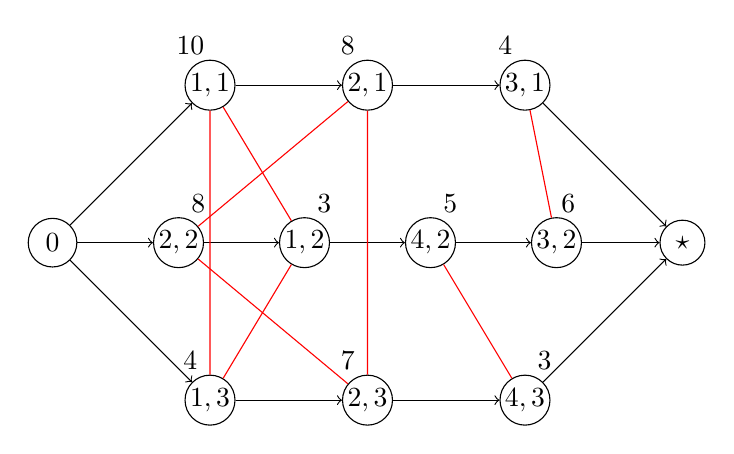
\begin{tikzpicture}              
            \node [circle, draw=black] (0) at (0, 0) {$0$}; 
            \node [circle, draw=black, inner sep=0.5pt] (11) at (2, 2) {$1, 1$}; 
            \node [circle, draw=black, inner sep=0.5pt] (21) at (4, 2) {$2, 1$}; 
            \node [circle, draw=black, inner sep=0.5pt] (31) at (6, 2) {$3, 1$}; 

            \node [circle, draw=black, inner sep=0.5pt] (22) at (1.6, 0) {$2, 2$}; 
            \node [circle, draw=black, inner sep=0.5pt] (12) at (3.2, 0) {$1, 2$};
            \node [circle, draw=black, inner sep=0.5pt] (42) at (4.8, 0) {$4, 2$};
            \node [circle, draw=black, inner sep=0.5pt] (32) at (6.4, 0) {$3, 2$};

            \node [circle, draw=black, inner sep=0.5pt] (13) at (2, -2) {$1, 3$}; 
            \node [circle, draw=black, inner sep=0.5pt] (23) at (4, -2) {$2, 3$}; 
            \node [circle, draw=black, inner sep=0.5pt] (43) at (6, -2) {$4, 3$};

            \node (p11) at (1.75, 2.5) {$10$}; 
            \node (p21) at (3.75, 2.5) {$8$}; 
            \node (p31) at (5.75, 2.5) {$4$}; 

            \node (p22) at (1.85, 0.5) {$8$};
            \node (p12) at (3.45, 0.5) {$3$}; 
            \node (p42) at (5.05, 0.5) {$5$}; 
            \node (p32) at (6.55, 0.5) {$6$}; 

            \node (p13) at (1.75, -1.5) {$4$}; 
            \node (p23) at (3.75, -1.5) {$7$};
            \node (p43) at (6.25, -1.5) {$3$};

            \node [circle, draw=black] (star) at (8, 0) {$\star$};
            
            \draw [->] (0) -- (11); \draw [->] (0) -- (22); \draw [->] (0) -- (13);
            \draw [->] (11) -- (21); \draw [->] (21) -- (31); \draw [->] (31) -- (star);
            \draw [->] (22) -- (12); \draw [->] (12) -- (42); \draw [->] (42) -- (32); \draw [->] (32) -- (star);
            \draw [->] (13) -- (23); \draw [->] (23) -- (43); \draw [->] (43) -- (star);

            \draw [color=red] (11) -- (12) -- (13) -- (11);
            \draw [color=red] (21) -- (22) -- (23) -- (21);
            \draw [color=red] (31) edge (32);
            \draw [color=red] (42) edge (43);
        \end{tikzpicture} 
    \end{center}
    Then applying Algorithm~\ref{algo:9.3} gives us 
    \begin{align*}
        \Omega &= \{(1, 1), (2, 2), (1, 3)\}, \\ 
        t(\Omega) &= \min\{0 + 10, 0 + 8, 0 + 4\} = 4, \\ 
        i^* &= 1, \\ 
        \Omega' &= \{(1, 1), (1, 3)\}. 
    \end{align*}
    So at level $1$, there are two nodes of interest: one corresponding to 
    operation $(1, 1)$ being processed first on machine $1$, and the other 
    corresponding to operation $(1, 3)$ being processed first on machine $1$.
    
    If operation $(1, 1)$ is scheduled first, we add directions to the 
    following blue disjunctive arcs to the graph. 
    \begin{center}
        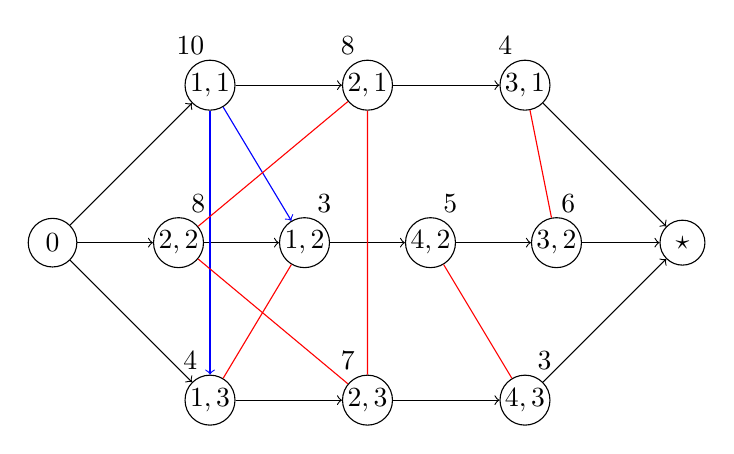
\begin{tikzpicture}              
            \node [circle, draw=black] (0) at (0, 0) {$0$}; 
            \node [circle, draw=black, inner sep=0.5pt] (11) at (2, 2) {$1, 1$}; 
            \node [circle, draw=black, inner sep=0.5pt] (21) at (4, 2) {$2, 1$}; 
            \node [circle, draw=black, inner sep=0.5pt] (31) at (6, 2) {$3, 1$}; 

            \node [circle, draw=black, inner sep=0.5pt] (22) at (1.6, 0) {$2, 2$}; 
            \node [circle, draw=black, inner sep=0.5pt] (12) at (3.2, 0) {$1, 2$};
            \node [circle, draw=black, inner sep=0.5pt] (42) at (4.8, 0) {$4, 2$};
            \node [circle, draw=black, inner sep=0.5pt] (32) at (6.4, 0) {$3, 2$};

            \node [circle, draw=black, inner sep=0.5pt] (13) at (2, -2) {$1, 3$}; 
            \node [circle, draw=black, inner sep=0.5pt] (23) at (4, -2) {$2, 3$}; 
            \node [circle, draw=black, inner sep=0.5pt] (43) at (6, -2) {$4, 3$};

            \node (p11) at (1.75, 2.5) {$10$}; 
            \node (p21) at (3.75, 2.5) {$8$}; 
            \node (p31) at (5.75, 2.5) {$4$}; 

            \node (p22) at (1.85, 0.5) {$8$};
            \node (p12) at (3.45, 0.5) {$3$}; 
            \node (p42) at (5.05, 0.5) {$5$}; 
            \node (p32) at (6.55, 0.5) {$6$}; 

            \node (p13) at (1.75, -1.5) {$4$}; 
            \node (p23) at (3.75, -1.5) {$7$};
            \node (p43) at (6.25, -1.5) {$3$};

            \node [circle, draw=black] (star) at (8, 0) {$\star$};
            
            \draw [->] (0) -- (11); \draw [->] (0) -- (22); \draw [->] (0) -- (13);
            \draw [->] (11) -- (21); \draw [->] (21) -- (31); \draw [->] (31) -- (star);
            \draw [->] (22) -- (12); \draw [->] (12) -- (42); \draw [->] (42) -- (32); \draw [->] (32) -- (star);
            \draw [->] (13) -- (23); \draw [->] (23) -- (43); \draw [->] (43) -- (star);

            \draw [->, color=blue] (11) -- (12);
            \draw [->, color=blue] (11) -- (13);
            \draw [color=red] (12) -- (13);
            \draw [color=red] (21) -- (22) -- (23) -- (21);
            \draw [color=red] (31) edge (32);
            \draw [color=red] (42) edge (43);
        \end{tikzpicture} 
    \end{center}
    This node is characterized by the two disjunctive arcs 
    $(1, 1) \to (1, 2)$ and $(1, 1) \to (1, 3)$. The addition of these 
    disjunctive arcs gives us a new longest path $0 \to (1, 1) \to (1, 2) 
    \to (4, 2) \to (3, 2) \to \star$ and a lower bound $\text{LB}(V') = 24$.
    In order to improve this lower bound, we can generate an instance of 
    $(1~|~r_j~|~L_{\max})$ for machine $1$. The release date of job $j$ 
    in this single machine problem is determined by the longest 
    path from the source node $0$ to the node $(1, j)$ excluding 
    the cost of node $(1, j)$, and the due date is computed by finding the 
    longest path from $(1, j)$ to the sink $\star$ (excluding the cost 
    of $(1, j)$ itself) and subtracting the resulting value from 
    $\text{LB}(V') = 24$. This leads us to the following instance 
    of $(1~|~r_j~|~L_{\max})$ for machine $1$. 
    \begin{align*}
        \begin{array}{c|ccc}
            j & 1 & 2 & 3 \\ \hline 
            p_{1j} & 10 & 3 & 4 \\ 
            r_{1j} & 0 & 10 & 10 \\ 
            d_{1j} & 10 & 13 & 14 
        \end{array}
    \end{align*}
    The sequence that minimizes $L_{\max}$ is $1, 2, 3$ with $L_{\max} = 3$, 
    implying that a lower bound for the makespan at the corresponding node 
    is $24 + 3 = 27$. We can also generate an instance of $(1~|~r_j~|~L_{\max})$ 
    for machine $2$ in the same way, and the release dates and due dates 
    are as follows. 
    \begin{align*}
        \begin{array}{c|ccc}
            j & 1 & 2 & 3 \\ \hline 
            p_{2j} & 8 & 8 & 7 \\ 
            r_{2j} & 10 & 0 & 14 \\ 
            d_{2j} & 20 & 10 & 21 
        \end{array}
    \end{align*}
    The optimal sequence is $2, 1, 3$ with $L_{\max} = 4$, so we get a 
    better lower bound of $24 + 4 = 28$ for the node with operation $(1, 1)$ 
    scheduled first. Analyzing machines $3$ and $4$ in the same way does not 
    yield a better lower bound. 

    The second node at level $1$ corresponds to operation $(1, 3)$ being scheduled
    first. In this case, we add the disjunctive arcs $(1, 3) \to (1, 1)$ 
    and $(1, 3) \to (1, 2)$ instead. 
    \begin{center}
        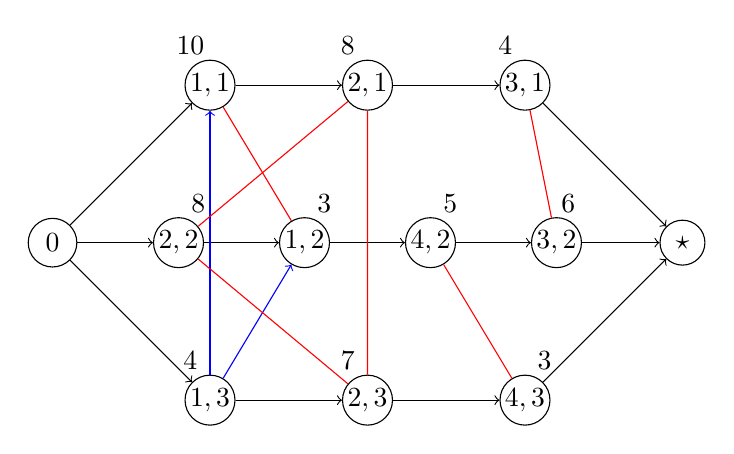
\begin{tikzpicture}              
            \node [circle, draw=black] (0) at (0, 0) {$0$}; 
            \node [circle, draw=black, inner sep=0.5pt] (11) at (2, 2) {$1, 1$}; 
            \node [circle, draw=black, inner sep=0.5pt] (21) at (4, 2) {$2, 1$}; 
            \node [circle, draw=black, inner sep=0.5pt] (31) at (6, 2) {$3, 1$}; 

            \node [circle, draw=black, inner sep=0.5pt] (22) at (1.6, 0) {$2, 2$}; 
            \node [circle, draw=black, inner sep=0.5pt] (12) at (3.2, 0) {$1, 2$};
            \node [circle, draw=black, inner sep=0.5pt] (42) at (4.8, 0) {$4, 2$};
            \node [circle, draw=black, inner sep=0.5pt] (32) at (6.4, 0) {$3, 2$};

            \node [circle, draw=black, inner sep=0.5pt] (13) at (2, -2) {$1, 3$}; 
            \node [circle, draw=black, inner sep=0.5pt] (23) at (4, -2) {$2, 3$}; 
            \node [circle, draw=black, inner sep=0.5pt] (43) at (6, -2) {$4, 3$};

            \node (p11) at (1.75, 2.5) {$10$}; 
            \node (p21) at (3.75, 2.5) {$8$}; 
            \node (p31) at (5.75, 2.5) {$4$}; 

            \node (p22) at (1.85, 0.5) {$8$};
            \node (p12) at (3.45, 0.5) {$3$}; 
            \node (p42) at (5.05, 0.5) {$5$}; 
            \node (p32) at (6.55, 0.5) {$6$}; 

            \node (p13) at (1.75, -1.5) {$4$}; 
            \node (p23) at (3.75, -1.5) {$7$};
            \node (p43) at (6.25, -1.5) {$3$};

            \node [circle, draw=black] (star) at (8, 0) {$\star$};
            
            \draw [->] (0) -- (11); \draw [->] (0) -- (22); \draw [->] (0) -- (13);
            \draw [->] (11) -- (21); \draw [->] (21) -- (31); \draw [->] (31) -- (star);
            \draw [->] (22) -- (12); \draw [->] (12) -- (42); \draw [->] (42) -- (32); \draw [->] (32) -- (star);
            \draw [->] (13) -- (23); \draw [->] (23) -- (43); \draw [->] (43) -- (star);

            \draw [->, color=blue] (13) -- (11);
            \draw [->, color=blue] (13) -- (12);
            \draw [color=red] (11) -- (12);
            \draw [color=red] (21) -- (22) -- (23) -- (21);
            \draw [color=red] (31) edge (32);
            \draw [color=red] (42) edge (43);
        \end{tikzpicture} 
    \end{center}
    We see that a lower bound on the makespan is $\text{LB}(V') = 26$ 
    via the longest path $0 \to (1, 3) \to (1, 1) \to (2, 1) \to (3, 1) 
    \to \star$. The associated maximum lateness problem for machine 
    $1$ has optimal sequence $3, 1, 2$ with $L_{\max} = 2$, which 
    implies that a lower bound for this node is $26 + 2 = 28$. Analyzing
    machines $2$, $3$, and $4$ in this way does not result in a better lower 
    bound. 

    The next step is to branch from node $(1, 1)$ at level $1$. Applying 
    Algorithm~\ref{algo:9.3} yields 
    \begin{align*}
        \Omega &= \{(2, 2), (2, 1), (1, 3)\}, \\ 
        t(\Omega) &= \min(0 + 8, 10 + 8, 10 + 4) = 8, \\ 
        i^* &= 2, \\ 
        \Omega' &= \{(2, 2)\}. 
    \end{align*}
    There is one node of interest at level 2, namely the node corresponding to 
    operation $(2, 2)$ being processed first on machine $2$. We add the
    disjunctive arcs $(2, 2) \to (2, 1)$ and $(2, 2) \to (2, 3)$ to the graph. 
    \begin{center}
        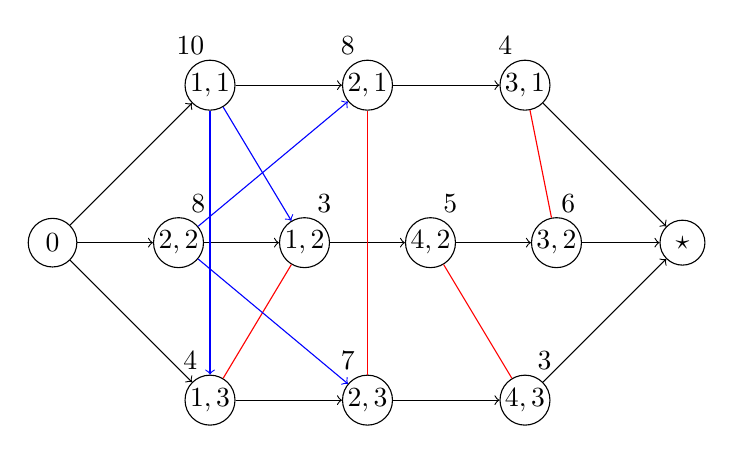
\begin{tikzpicture}              
            \node [circle, draw=black] (0) at (0, 0) {$0$}; 
            \node [circle, draw=black, inner sep=0.5pt] (11) at (2, 2) {$1, 1$}; 
            \node [circle, draw=black, inner sep=0.5pt] (21) at (4, 2) {$2, 1$}; 
            \node [circle, draw=black, inner sep=0.5pt] (31) at (6, 2) {$3, 1$}; 

            \node [circle, draw=black, inner sep=0.5pt] (22) at (1.6, 0) {$2, 2$}; 
            \node [circle, draw=black, inner sep=0.5pt] (12) at (3.2, 0) {$1, 2$};
            \node [circle, draw=black, inner sep=0.5pt] (42) at (4.8, 0) {$4, 2$};
            \node [circle, draw=black, inner sep=0.5pt] (32) at (6.4, 0) {$3, 2$};

            \node [circle, draw=black, inner sep=0.5pt] (13) at (2, -2) {$1, 3$}; 
            \node [circle, draw=black, inner sep=0.5pt] (23) at (4, -2) {$2, 3$}; 
            \node [circle, draw=black, inner sep=0.5pt] (43) at (6, -2) {$4, 3$};

            \node (p11) at (1.75, 2.5) {$10$}; 
            \node (p21) at (3.75, 2.5) {$8$}; 
            \node (p31) at (5.75, 2.5) {$4$}; 

            \node (p22) at (1.85, 0.5) {$8$};
            \node (p12) at (3.45, 0.5) {$3$}; 
            \node (p42) at (5.05, 0.5) {$5$}; 
            \node (p32) at (6.55, 0.5) {$6$}; 

            \node (p13) at (1.75, -1.5) {$4$}; 
            \node (p23) at (3.75, -1.5) {$7$};
            \node (p43) at (6.25, -1.5) {$3$};

            \node [circle, draw=black] (star) at (8, 0) {$\star$};
            
            \draw [->] (0) -- (11); \draw [->] (0) -- (22); \draw [->] (0) -- (13);
            \draw [->] (11) -- (21); \draw [->] (21) -- (31); \draw [->] (31) -- (star);
            \draw [->] (22) -- (12); \draw [->] (12) -- (42); \draw [->] (42) -- (32); \draw [->] (32) -- (star);
            \draw [->] (13) -- (23); \draw [->] (23) -- (43); \draw [->] (43) -- (star);

            \draw [->, color=blue] (11) -- (12);
            \draw [->, color=blue] (11) -- (13);
            \draw [color=red] (12) -- (13);
            \draw [->, color=blue] (22) -- (21);
            \draw [->, color=blue] (22) -- (23); 
            \draw [color=red] (21) -- (23);
            \draw [color=red] (31) edge (32);
            \draw [color=red] (42) edge (43);
        \end{tikzpicture} 
    \end{center}
    We have a lower bound $\text{LB}(V') = 28$ on this node because the 
    preceding node had this lower bound. This leads to an instance of 
    $(1~|~r_j~|~L_{\max})$ for machine $1$ with the following release 
    dates and due dates. 
    \begin{align*}
        \begin{array}{c|ccc}
            j & 1 & 2 & 3 \\ \hline 
            p_{1j} & 10 & 3 & 4 \\ 
            r_{1j} & 0 & 10 & 10 \\ 
            d_{1j} & 14 & 17 & 18 
        \end{array}
    \end{align*}
    The optimal sequence is $1, 3, 2$ with $L_{\max} = 0$. Then a 
    lower bound on this node is also $28 + 0 = 28$, and analyzing 
    machines $2$, $3$, and $4$ in the same way does not increase the 
    lower bound. 

    So far, the branch and bound tree is as follows. 
    \begin{center}
        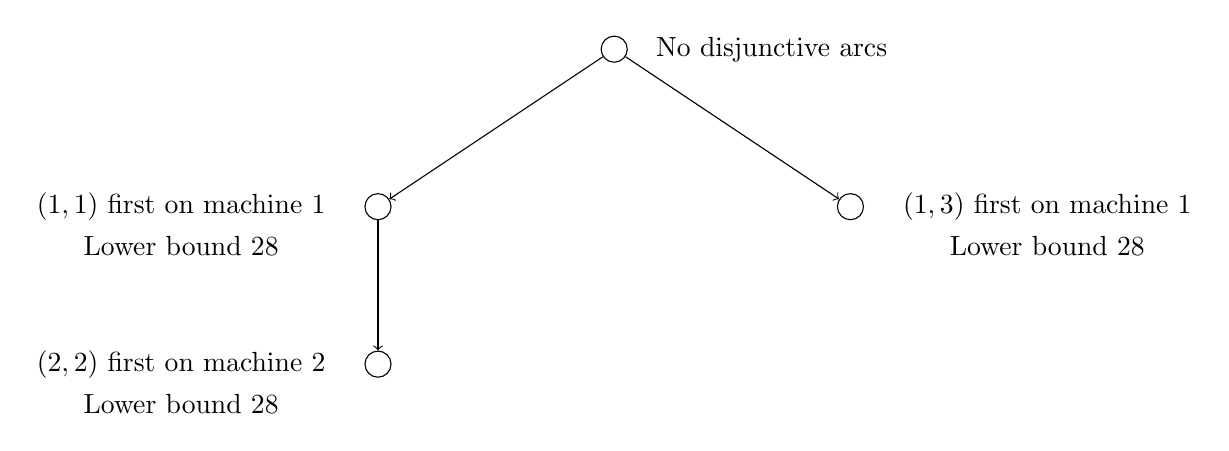
\begin{tikzpicture}              
            \node [circle, draw=black] (BB0) at (3, 8) {}; 
            \node [circle, draw=black] (BB11) at (0, 6) {}; 
            \node [circle, draw=black] (BB13) at (6, 6) {}; 
            \node [circle, draw=black] (BB22) at (0, 4) {};
            \node (DBB0) at (5, 8) {No disjunctive arcs}; 
            \node (DBB111) at (-2.5, 6) {$(1, 1)$ first on machine $1$};
            \node (DBB112) at (-2.5, 5.5) {Lower bound 28}; 
            \node (DBB131) at (8.5, 6) {$(1, 3)$ first on machine $1$};
            \node (DBB132) at (8.5, 5.5) {Lower bound 28}; 
            \node (DBB221) at (-2.5, 4) {$(2, 2)$ first on machine $2$};
            \node (DBB222) at (-2.5, 3.5) {Lower bound 28}; 
            
            \draw [->] (BB0) -- (BB11);
            \draw [->] (BB0) -- (BB13);
            \draw [->] (BB11) -- (BB22);
        \end{tikzpicture} 
    \end{center}
    Continuing the branch and bound procedure results in the following job 
    sequence for the four machines. 
    \begin{align*}
        \begin{array}{c|c}
            \text{Machine} & \text{Job Sequence} \\ \hline 
            1 & 1, 3, 2 \text{ or } 1, 2, 3 \\ 
            2 & 2, 1, 3 \\ 
            3 & 1, 2 \\ 
            4 & 2, 3
        \end{array}
    \end{align*}
    The makespan under this schedule is $28$, as seen in the following Gantt chart. 
    \begin{center} 
        \begin{tikzpicture}[/pgfgantt/y unit chart=0.65cm] 
            \begin{ganttchart}[
                title/.style={draw=none},
                canvas/.append style={draw=none}, 
                bar top shift=0.1, bar height=0.6,
                y unit title=0.65cm,
                x unit=0.4cm
            ]{1}{28}
                \ganttbar{Machine 1}{1}{10} \ganttbar[inline]{1}{1}{10} \ganttbar[inline]{3}{11}{14} \ganttbar[inline]{2}{15}{17} \\ 
                \ganttbar{Machine 2}{1}{8} \ganttbar[inline]{2}{1}{8} \ganttbar[inline]{1}{11}{18} \ganttbar[inline]{3}{19}{25} \\ 
                \ganttbar{Machine 3}{19}{22} \ganttbar[inline]{1}{19}{22} \ganttbar[inline]{2}{23}{28} \\ 
                \ganttbar{Machine 4}{18}{22} \ganttbar[inline]{1}{18}{22} \ganttbar[inline]{3}{26}{28} \\ 
                \gantttitlelist{1,...,28}{1}
            \end{ganttchart}
        \end{tikzpicture}
    \end{center} 
    \vspace{-0.4cm}
\end{exmp}

While this approach is guaranteed to lead to an optimal schedule, the 
computation time is prohibitive with a large number of machines and a large 
number of jobs. With $20$ machines and $20$ jobs, it is already hard to 
find an optimal schedule. It is therefore necessarily to develop heuristics 
that lead to reasonably good schedules in a reasonably short time. The 
next section describes a well-known heuristic with an excellent track record.

\subsection{The Shifting Bottleneck Heuristic for Makespan} \label{subsec:9.2}
One of the most successful heuristic procedures developed for $(J_m~||~C_{\max})$ 
is the {\bf Shifting Bottleneck} heuristic. We denote the set of all 
machines by $M$. In the description of an iteration of the heuristic, 
it is assumed that in previous iterations, a selection of disjunctive 
arcs has already been fixed for a subset $M_0$ of machines. So for each 
of the machines in $M_0$, a sequence of operations has already been determined. 

An iteration determines which machine in $M \setminus M_0$ has to be included 
next into $M_0$. The sequence in which the operations on this machine 
have to be processed is also generated in this iteration. 

In order to select the machine to be included next in $M_0$, an attempt is 
made to determine which one of the machines yet to be scheduled would cause in 
some sense the severest disruption. To determine this, we consider the 
graph with only the directions of the disjunctive arcs of the machines in $M_0$
fixed. Call this graph $G'$. For the machines in $M \setminus M_0$, having 
no directions fixed on the disjunctive arcs implies that all operations 
on this machine can be done in parallel (as if the machine has infinite 
capacity, or equivalently, each one of the operations has the machine 
for itself). The graph $G'$ has one or more critical paths that determine 
the corresponding makespan. Call this makespan $C_{\max}(M_0)$. 

Let $i \in M \setminus M_0$, and suppose that operation $(i, j)$ has to be 
processed at a time window in which the release date and due date are 
determined by the critical (longest) paths in $G'$. That is, the 
release date is equal to the longest path in $G'$ from the source node $0$ 
to node $(i, j)$ (excluding the cost of $(i, j)$ itself), and the 
due date is equal to $C_{\max}(M_0)$ minus the longest path from 
node $(i, j)$ to the sink node $\star$ (again excluding the cost of 
$(i, j)$ itself). Then we can consider for each machine in $M \setminus M_0$ 
a separate $(1~|~r_j~|~L_{\max})$ problem. We stated earlier that this 
is strongly $\NP$-hard, but there are procedures that perform reasonably well.
The minimum $L_{\max}$ of the single machine problem corresponding to 
machine $i$ is denoted by $L_{\max}(i)$ and is a measure of the criticality of 
machine $i$. 

After solving all these single machine problems, the machine with the 
\emph{largest} maximum lateness is chosen. Among the remaining machines, 
this machine is in a sense the most critical or the ``bottleneck'' and therefore 
the one to be included next in $M_0$. Label this machine $k$, call its 
maximum lateness $L_{\max}(k)$, and schedule it according to the optimal 
solution obtained for the single machine problem associated with this 
machine. If the disjunctive arcs that specify the sequence of operations on 
machine $k$ are inserted in graph $G'$, then the makespan
of the current partial schedule increases by at least $L_{\max}(k)$; that is,
\[ C_{\max}(M_0 \cup \{k\}) \geq C_{\max}(M_0) + L_{\max}(k). \] 
Before starting the next iteration and determining the next machine to be
scheduled, one additional step has to be done within the current iteration. In
this additional step, all the machines in the original set $M_0$ are 
resequenced in order to see if the makespan can be reduced. That is, 
a machine, say $\ell$, is taken out of $M_0$ and a graph $G''$ is 
constructed by modifying $G'$ through the inclusion of the disjunctive arcs 
that specify the sequence of operations on machine $k$ and the exclusion 
of the disjunctive arcs associated with machine $\ell$. Then machine $\ell$ 
is resequenced by solving the corresponding $(1~|~r_j~|~L_{\max})$ 
problem with the release and due dates determined by the critical paths in 
$G''$. Resequencing each of the machines in the original set $M_0$ completes 
the iteration. 

Afterwards, the entire procedure is repeated and another machine is added 
to the current set $M_0 \cup \{k\}$. We summarize the algorithm as follows. 

\begin{algo}[Shifting Bottleneck Heuristic]{algo:9.5}
    \begin{enumerate}
        \item {\bf Initial conditions.} Set $M_0 = \varnothing$. The graph $G$ 
        has all the conjunctive arcs and no directions on the disjunctive arcs. 
        Set $C_{\max}(M_0)$ equal to the longest path in $G$. 

        \item {\bf Analysis of machines yet to be scheduled.} For each 
        machine in $M \setminus M_0$, do the following: 
        \begin{enumerate}[(a)]
            \item Generate an instance of $(1~|~r_j~|~L_{\max})$ with the 
            release date of operation $(i, j)$ determined by the longest 
            path in $G$ from the source node $0$ to node $(i, j)$ 
            (excluding $p_{ij}$), and the due date of operation $(i, j)$ 
            determined by $C_{\max}(M_0)$ minus the longest path in $G$ 
            from node $(i, j)$ to the sink $\star$ (excluding $p_{ij}$).
            \item Minimize $L_{\max}$ in each of these single machine 
            subproblems, and let $L_{\max}(i)$ denote the minimum 
            $L_{\max}$ in the subproblem corresponding to machine $i$. 
        \end{enumerate}

        \item {\bf Bottleneck selection and sequencing.} Let 
        \[ L_{\max}(k) = \max_{i \in M \setminus M_0} L_{\max}(i). \] 
        Sequence machine $k$ according to the sequence obtained in Step 2 
        for that machine. Insert all the corresponding disjunctive arcs 
        in $G$, and insert machine $k$ in $M_0$. 

        \item {\bf Resequencing of all earlier scheduled machines.} 
        For each machine $i \in M_0 \setminus \{k\}$, do the following: 
        \begin{enumerate}[(a)]
            \item Delete from $G$ the disjunctive arcs corresponding to machine $i$. 
            \item Formulate a $(1~|~r_j~|~L_{\max})$ subproblem for machine $i$ 
            with release dates and due dates of the operations determined by the 
            longest path calculations in $G$.
            \item Find the sequence which minimizes $L_{\max}(i)$ and insert the 
            corresponding disjunctive arcs in $G$. 
        \end{enumerate}

        \item {\bf Stopping criterion.} If $M_0 = M$, then stop. Otherwise, go back 
        to Step 2. 
    \end{enumerate}
\end{algo}

The structure of the shifting bottleneck heuristic shows the relationship between 
the bottleneck concept and more combinatorial concepts such as critical
(longest) path and maximum lateness. A critical path indicates the location
and the timing of a bottleneck. The maximum lateness gives an indication of
the amount by which the makespan increases if a machine is added to the set
of machines already scheduled.

Extensive numerical research has shown that the Shifting Bottleneck heuristic is extremely 
effective. When applied to a standard test problem with $10$
machines and $10$ jobs that had remained unsolved for more than $20$ years, the
heuristic obtained a very good solution very fast. This solution turned out to
be optimal after a branch and bound procedure found the same result and verified its 
optimality. The branch and bound approach, in contrast to the heuristic,
needed many hours of CPU time. The disadvantage of the heuristic is, of course,
that there is no guarantee that the solution it reaches is optimal.